\chapter{Number 3}
\section{Speical Sequences}
We have looked at sequences previously.  In this chapter we will look at the properties of some sequences and use these to find the formulae of related patterns.  Things we can look at are the nature of the numbers in the sequence, are they odd or even, is there a pattern between the gaps in the terms and anything else we might see.
\subsection{Square Numbers}
Let's consider a pattern of squares made up of dots.

\bigskip
  \begin{center}
    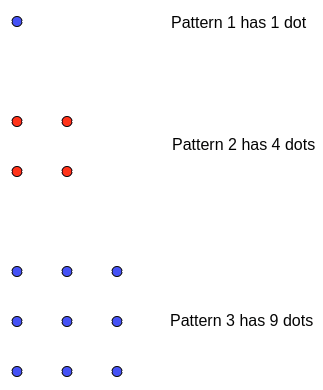
\includegraphics[scale=0.5]{./Images/Sequences/Seq_1.png}
  \end{center}
\bigskip

To calculate the number of dots in a pattern we multiply the number of dots along by the number of dots up.  Since the number of dots up and along is equal to the pattern number we can say that we square the pattern number.

\subsubsection{Exercise}
Calculate the value of the first 15 square numbers.  The first three square numbers are:
\begin{enumerate}
  \item $1 \times 1 \rightarrow 1$
  \item $2 \times 2 \rightarrow 4$
  \item $3 \times 3 \rightarrow 9$
  \item ...
\end{enumerate}

\subsubsection{Exercise}
The first 5 terms are 1, 4, 9, 16, 25...

The difference between the 1st and 2nd terms is 3.

The difference between the 2nd and 3rd terms is 5.

Find the difference between the terms for the first 10 terms and describe this new pattern of numbers.

Now find the diffences for this sequence.

\subsubsection{Square Numbers Formula}
A formula that generates the sequence of square numbers is $n^{th} = n^2$

Verify that this formula gives the first 5 terms.

\subsubsection{Exercise}
Let's consider the sequence generated with the formula $n^{th}=2n^2$
\begin{enumerate}
  \item Write down the first ten terms for the sequence.  The first two are 2 and 8.
  \item Find the differences between the terms.
  \item Describe what you notice.
  \item Find the difference between the terms for this new pattern. (We call this the second difference)
\end{enumerate}

\subsubsection{Exercise}
Do as we did for the previous exercise for the following sequences.  Pay careful attention to the answers you get because they will be needed for the questions at the end of the exercise.
\begin{enumerate}
  \item $n^{th}=2n^2 + 5$
  \item $n^{th}=2n^2 + n$
  \item $n^{th}=3n^2$
  \item $n^{th}=3n^2-4$
  \item $n^{th}=3n^2+5n$
  \item $n^{th}=4n^2$
  \item $n^{th}=5n^2$
  \item If the second difference of a sequence is always 6, what can you say about the sequence?
  \item If the second difference of a sequence is always 12, what can you say about the sequence?
  \item If the second difference of a sequence is always 16, what can you say about the sequence?
\end{enumerate}


\subsection{Triangular numbers}
Let's consider a pattern of triangles made up of dots.

\bigskip
  \begin{center}
    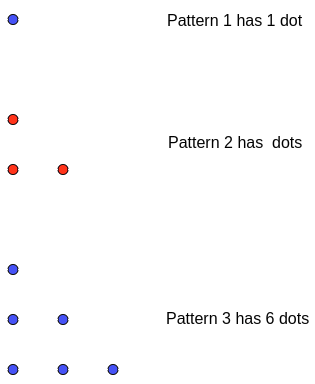
\includegraphics[scale=0.5]{./Images/Sequences/Seq_2.png}
  \end{center}
\bigskip

\subsubsection{Exercise}
Find the first and second differences for the triangular numbers.
Note that any sequence with the same second difference is going to be related to the triangular numbers.

\subsubsection{Formulae for genterating triangular numbers}
All sequence with a second difference of 1 will have the formula

\bigskip
  $\displaystyle n^{th}=\frac{n}{2}(n + 1)$
\bigskip

Consider the sequence 2, 4, 7, 11, 16, ...

We can see that this has a second difference of 1 so  it is related to the triangular numbers.  On close inspection we can see that all of our nummbers are one more so this must be the sequence generated by the formula:

\bigskip
  $\displaystyle n^{th}=\frac{n}{2}(n + 1) + 1$
\bigskip

\subsubsection{Exercise}
Each of the sequences below are related to the sequeces of the forms:

$an^2 + b$ or $\displaystyle n^{th}=\frac{n}{2}(n + 1) + a$

Find the equation that generates theoremstyle

\begin{enumerate}
  \item 1, 3, 6, 10, ...
  \item 1, 4, 9, 16, ...
  \item 3, 5, 8, 12, ...
  \item 3, 12, 27, 48, ...
  \item 0, 2, 5, 9, ...
  \item 0, 3, 8, 15, ...
\end{enumerate}

\subsubsection{Vector Motor Racing}
This game uses translations that we learnt about in the last chapter and is a lot of fun.  After you have played it for a while you might see that a knowledge of triangular numbers gives you an advantage.

The game is played on a grid and the cars move from point to point.  We use translations to give the cars speed and direction at any position.  We will use a vector to describe the translation, where the top number tells us how the car moved horizontally and the bottom number tells us how the car moves vertically.  The starting vector is:

\bigskip

$\left(
\begin{array}{c}
0\\
0\\
\end{array}
\right)$

\bigskip

This means that we are not moving across and we are not moving up.  We can change, if we choose, each of the numbers by '1', so that means that the top and botom numbers could each take on values of -1, 0 or 1.

Let's see how the first few moves could look for an individual car.

\bigskip
\begin{center}
  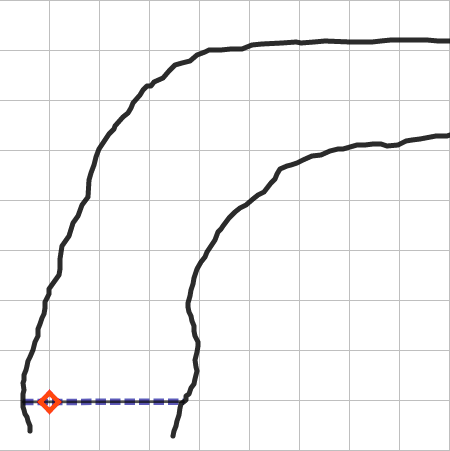
\includegraphics[scale=0.6]{./Images/Sequences/VMR_1.png}
\end{center}

We clearly want to move up and right so I will, for my first move, increase each value by 1 to get:

\bigskip

$\left(
\begin{array}{c}
1\\
1\\
\end{array}
\right)$

\bigskip

This will move the car to the point shown:

\bigskip
\begin{center}
  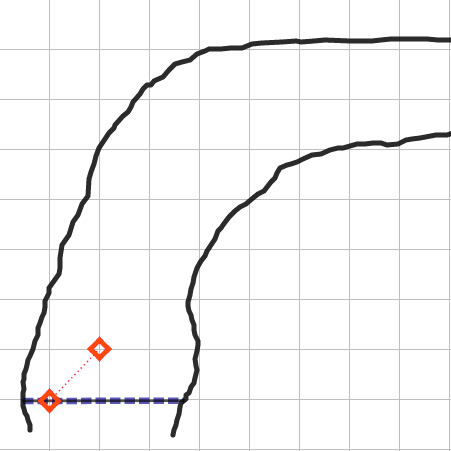
\includegraphics[scale=0.6]{./Images/Sequences/VMR_2.png}
\end{center}

The next two moves might go:

$\left(
\begin{array}{c}
1\\
2\\
\end{array}
\right)$
then
$\left(
\begin{array}{c}
2\\
2\\
\end{array}
\right)$

This would leave us in the position:

\bigskip
\begin{center}
  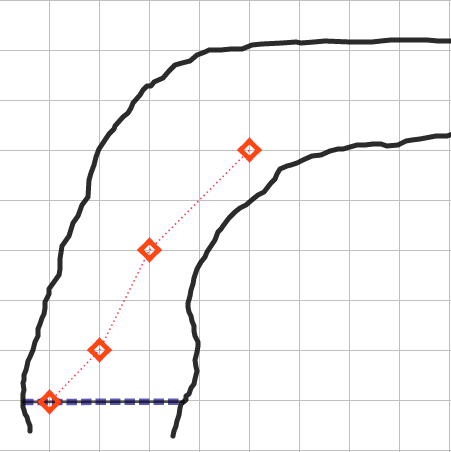
\includegraphics[scale=0.6]{./Images/Sequences/VMR_3.png}
\end{center}

When you play the game you will not be the only car.
Rules:
\begin{itemize}
  \item Players take it in turns
  \item You cannot end up in a position where there is already a car
  \item If you go off the track that is a crash and you are out
\end{itemize}
\subsection{Investigations}
\section{Primes}
There are different ways of describing numbers.  You have already come across odd and even numbers, now we are going to introduce prime numbers.  This is important because prime numbers are considered the building blocks of the number system.

Prime numbers are numbers with exactly 2 factors, so for example 3 is a prime number because its factors are 1 and 3, whereas 6 is not prime because it has factors 1, 2, 3 and 6.
The first five prime numbers are:

\bigskip

2, 3, 5, 7, 11, ...

\bigskip

A method we can use to find prime numbers is Eratosthenes grid

Steps:
\begin{enumerate}
  \item Make a square grid of numbers (e.g. 10 by 10)
  \item Cross out number 1
  \item Circle the first number not crossed out or already circled
  \item Cross out every multiple of that number
  \item If every number in the 1st row is crossed out or circled, circle all the numbers which are left and END
  \item Go back to step 3
\end{enumerate}

All the circled numbers are primes.

\subsubsection{Exercise}
Find all the prime numbers below 144

\subsection{Prime factor form}
We can write a number as an expression.  For example we could write 20 as $2 + 18$,  the problem is that this would not be unique.  However, if we write a number as just prime numbers multipled together then there is only one way to do this.

\bigskip

So for instance the only way to write 12 as a product of primes is $2 \times 2 \times 3$

We could write it in a different order, but this would be basically the same thing.
\subsection{Infinite primes}
